\documentclass{article}

\usepackage{xltxtra} % Loads fontspec, xunicode, metalogo, fxltx2e, and some extra customizations for XeLaTeX
%\defaultfontfeatures{Mapping=tex-text} % to support TeX conventions like ``---''
\defaultfontfeatures{Mapping=tex-text}
\setmainfont{Cambria}
\usepackage{csquotes}
\usepackage{graphicx}
\usepackage[margin=2.5cm]{geometry}
\newcounter{framenumber}
\setcounter{framenumber}{0}
%This command numbers frames and creates two blank lines for annotations.
\newcommand{\Annotate}{\stepcounter{framenumber}[\arabic{framenumber}]
\rule{\linewidth}{1pt}\\
\rule{\linewidth}{1pt}
\vspace{2\baselineskip}
\vfill
}
%Toggle to change the language of the subtitles.
%\newcommand{\Bislama}[1]{#1}
\newcommand{\Bislama}[1]{}
\newcommand{\English}[1]{#1}
%\newcommand{\English}[1]{}

\begin{document}
\center 
{\huge Tomato and Pumpkin} 
\vfill

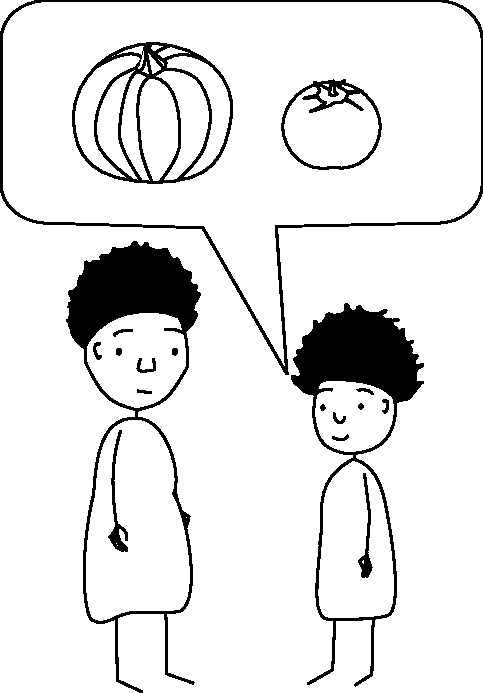
\includegraphics[scale=.7]{TomatoAndPumpkin01}

\Bislama{Hemia Yokon wetem anti blong hem, nem blong hem Rena. Yokon hemi se: "Mi wantem kakae tamat mo bamken."}
\English{This is Mutha and her mukul Bugulmana. Mutha says: "I want to eat some tomato and pumpkin."}

\Annotate

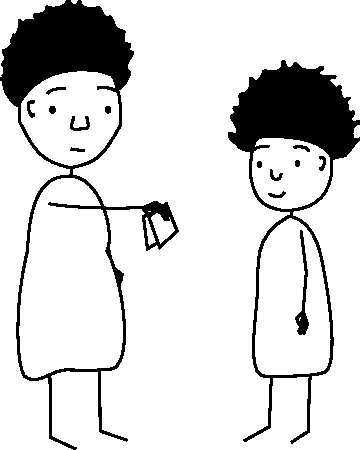
\includegraphics[scale=.6]{TomatoAndPumpkin02}

\Bislama{Rena hemi givim hem sids blong tamat mo bamken mo hemi talem hem blong planem.}
\English{Mukul gives her tomato and pumpkin seeds and tells her to plant them.}

\Annotate

\pagebreak

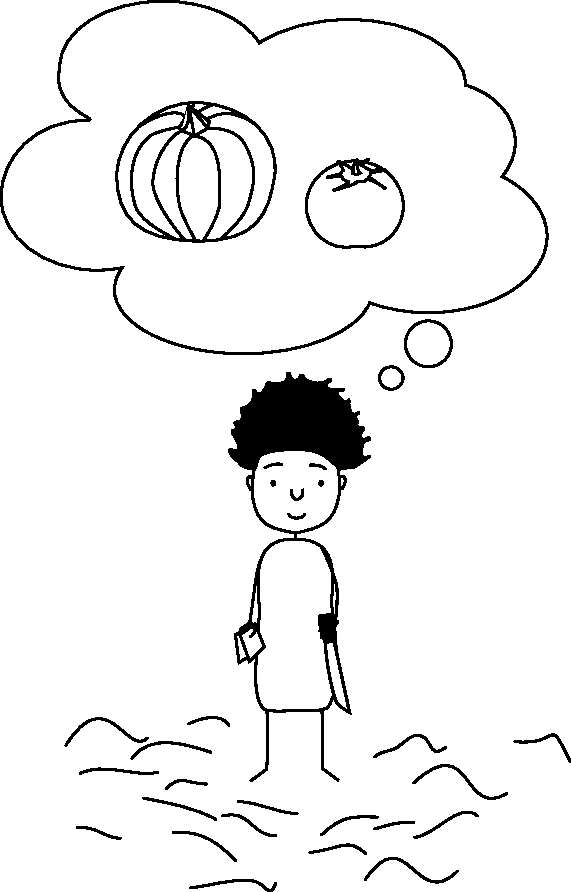
\includegraphics[scale=.6]{TomatoAndPumpkin03}

\Bislama{Yokon hemi planem sids ia.}
\English{Mutha plants the seeds. }

\Annotate

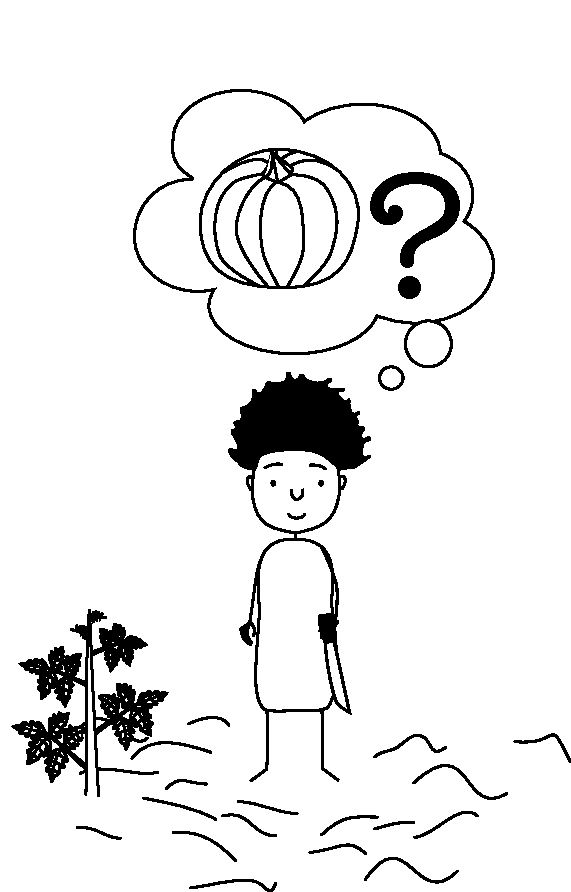
\includegraphics[scale=.5]{TomatoAndPumpkin04.pdf}

\Bislama{Wet gogo, ale wan stampa blong tamat hemi gru finis. Ale Yokon hemi stap tingbaot bamken.}
\English{After a while, a tomato plant has grown, but no pumpkin.}

\Annotate

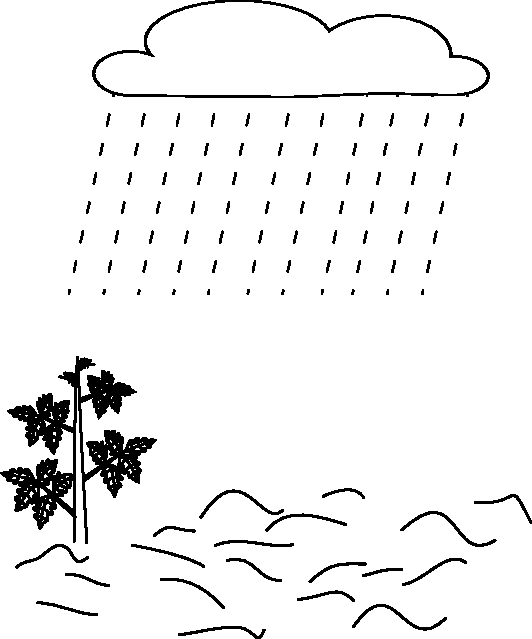
\includegraphics[scale=.6]{TomatoAndPumpkin05.pdf}

\Bislama{Ale ren i ren.}
\English{Then, there is rainfall.}

\Annotate

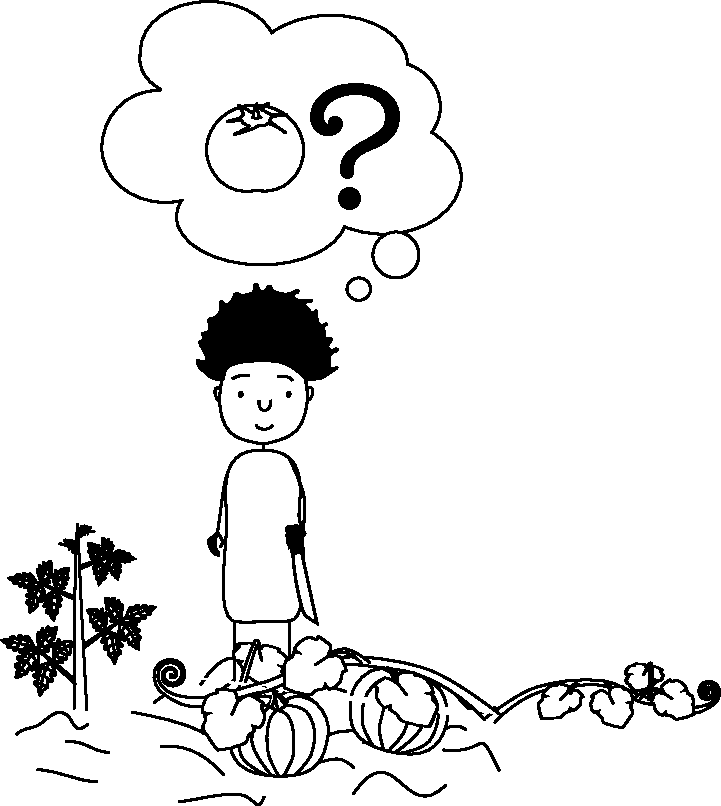
\includegraphics[scale=.6]{TomatoAndPumpkin06.pdf}

\Bislama{Wet gogo, bamken tu hemi gru finis, ale hemi karem frut finis. Be frut blong tamat hemi no stap yet.}
\English{Then, the pumpkin plant has also grown and it already bears pumpkins, but the tomato plant does not yet bear fruit.}

\Annotate

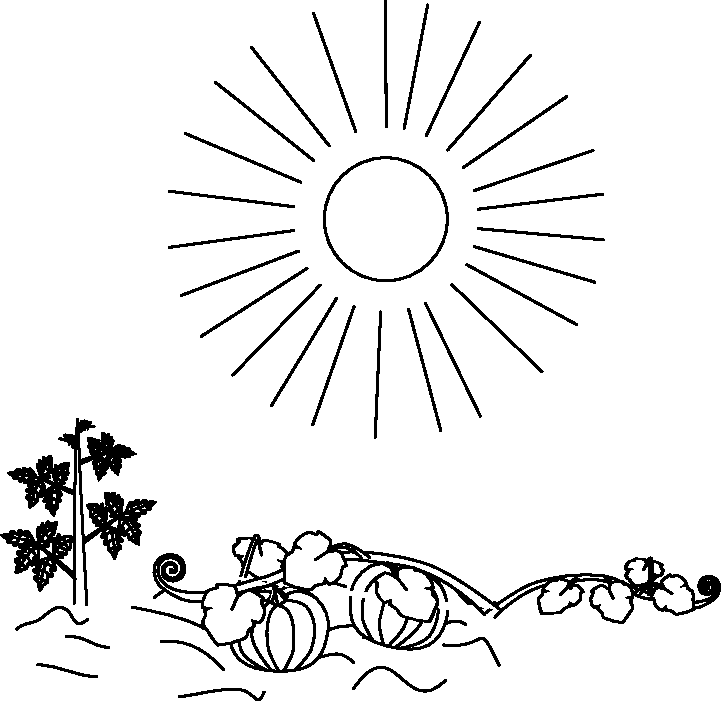
\includegraphics[scale=.6]{TomatoAndPumpkin07.pdf}

\Bislama{Afta, san i saen gud.}
\English{Then the sun comes out and shines brightly.}

\Annotate

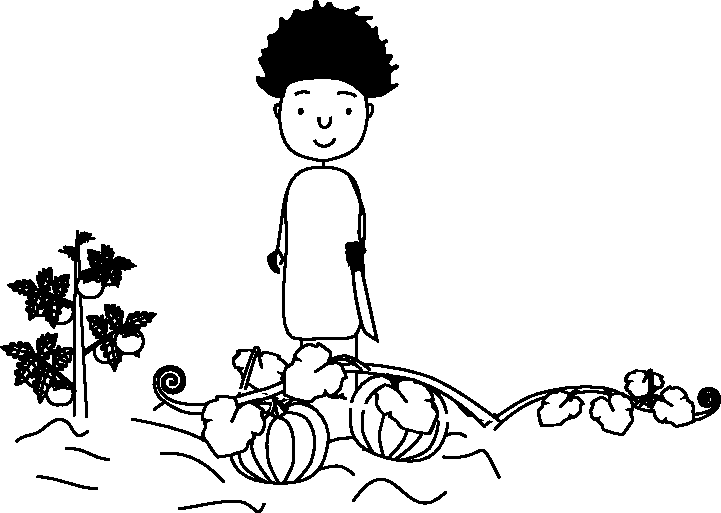
\includegraphics[scale=.7]{TomatoAndPumpkin08.pdf}

\Bislama{Wet gogo, ale stampa blong tamat tu hemi karem frut nao. Yokon hemi harem gud nao.}
\English{After some time, the tomato plant also bears fruit. Mutha is happy.}

\Annotate



\end{document}